\documentclass[
11pt, % The default document font size, options: 10pt, 11pt, 12pt
%codirector, % Uncomment to add a codirector to the title page
]{charter} 


% El títulos de la memoria, se usa en la carátula y se puede usar el cualquier lugar del documento con el comando \ttitle
\titulo{Sistema IoT para el monitoreo de niveles de ruido en entornos cerrados o pequeñas áreas urbanas} 

% Nombre del posgrado, se usa en la carátula y se puede usar el cualquier lugar del documento con el comando \degreename
\posgrado{Carrera de Especialización en Internet de las Cosas} 
%\posgrado{Carrera de Especialización en Internet de las Cosas} 
%\posgrado{Carrera de Especialización en Inteligencia Artificial}
%\posgrado{Maestría en Sistemas Embebidos} 
%\posgrado{Maestría en Internet de las cosas}

% Tu nombre, se puede usar el cualquier lugar del documento con el comando \authorname
% IMPORTANTE: no omitir titulaciones ni tildación en los nombres, también se recomienda escribir los nombres completos (tal cual los tienen en su documento)
\autor{Ing. José Pedro Rivero Peña}

% El nombre del director y co-director, se puede usar el cualquier lugar del documento con el comando \supname y \cosupname y \pertesupname y \pertecosupname
\director{Mgtr. Ing. Rodolfo Raúl Terán Aiza}
\pertenenciaDirector{UMSS} 
\codirector{} % para que aparezca en la portada se debe descomentar la opción codirector en los parámetros de documentclass
\pertenenciaCoDirector{FIUBA}

% Nombre del cliente, quien va a aprobar los resultados del proyecto, se puede usar con el comando \clientename y \empclientename
\cliente{          }
\empresaCliente{}
 
\fechaINICIO{04 de marzo de 2025}		%Fecha de inicio de la cursada de GdP \fechaInicioName
\fechaFINALPlan{22 de abril de 2025} 	%Fecha de final de cursada de GdP
\fechaFINALTrabajo{31 de octubre de 2025}	%Fecha de defensa pública del trabajo final


\begin{document}

\maketitle
\thispagestyle{empty}
\pagebreak


\thispagestyle{empty}
{\setlength{\parskip}{0pt}
\tableofcontents{}
}
\pagebreak


\section*{Registros de cambios}
\label{sec:registro}


\begin{table}[ht]
\label{tab:registro}
\centering
\begin{tabularx}{\linewidth}{@{}|c|X|c|@{}}
\hline
\rowcolor[HTML]{C0C0C0} 
Revisión & \multicolumn{1}{c|}{\cellcolor[HTML]{C0C0C0}Detalles de los cambios realizados} & Fecha      \\ \hline
0      & Creación del documento                                 &\fechaInicioName \\ \hline
1      & Se completa hasta el punto 5 inclusive                & {20} de {marzo} de 2025 \\ \hline
2      & Se completa hasta el punto 9 inclusive                & {28} de {marzo} de 2025 \\ \hline
3      & Se completa hasta el punto 12 inclusive                & {06} de {abril} de 2025 \\ \hline
4      & Se completa el plan	                                 & {11} de {abril} de 2025 \\ \hline
5      & Se corrigen observaciones	                                 & {19} de {abril} de 2025 \\ \hline

% Si hay más correcciones pasada la versión 4 también se deben especificar acá

\end{tabularx}
\end{table}

\pagebreak



\section*{Acta de constitución del proyecto}
\label{sec:acta}

\begin{flushright}
Buenos Aires, \fechaInicioName
\end{flushright}

\vspace{2cm}

Por medio de la presente se acuerda con el \authorname\hspace{1px} que su Trabajo 
Final de la \degreename\hspace{1px} se titulará ``\ttitle'' y consistirá en la implementación de un prototipo de un sistema 
IoT para el monitoreo de niveles de ruido en entornos cerrados o pequeñas áreas urbanas. El trabajo tendrá un presupuesto 
preliminar estimado de {620} horas y un costo estimado de ARS 8.347.200, con fecha de inicio el \fechaInicioName\hspace{1px} 
y fecha de presentación pública en octubre de 2025.

Se adjunta a esta acta la planificación inicial.

\vfill

% Esta parte se construye sola con la información que hayan cargado en el preámbulo del documento y no debe modificarla
\begin{table}[ht]
\centering
\begin{tabular}{ccc}
\begin{tabular}[c]{@{}c@{}}Dr. Ing. Ariel Lutenberg \\ Director posgrado FIUBA\end{tabular} & \hspace{2cm} & \begin{tabular}[c]{@{}c@{}}\clientename \\ \empclientename \end{tabular} \vspace{2.5cm} \\ 
\multicolumn{3}{c}{\begin{tabular}[c]{@{}c@{}} \supname \\ Director del Trabajo Final\end{tabular}} \vspace{2.5cm} \\
\end{tabular}
\end{table}




\section{1. Descripción técnica-conceptual del proyecto a realizar}
\label{sec:descripcion}

El monitoreo de los niveles acústicos en entornos cerrados y pequeños espacios urbanos es un problema que no se puede dejar de
 lado en la sociedad actual. La exposición constante a altos niveles de ruido puede generar estrés, fatiga auditiva y afectar 
 la concentración y productividad en oficinas, hospitales, aulas y parques. A pesar de la existencia de sistemas de medición 
 de ruidos, estos suelen ser costosos, estacionarios o requieren intervención manual para la toma y análisis de datos. En este 
 contexto, surge la necesidad de desarrollar soluciones tecnológicas accesibles, autónomas y escalables para la medición en 
 tiempo real de los niveles de ruido ambiental.

 Este proyecto propone el desarrollo de un sistema IoT capaz de monitorear el nivel de ruido en tiempo real, mediante sensores 
 que recopilan la información y la transmiten a una plataforma en la nube. De este modo, los usuarios pueden acceder a los 
 datos y gestionar alertas asociadas a parámetros definidos. A diferencia de soluciones tradicionales, esta propuesta se 
 enfoca en la modularidad y accesibilidad, permitiendo su implementación en diversos entornos sin necesidad de grandes 
 inversiones en infraestructura.
 La solución contempla el uso de sensores calibrados, microcontroladores con conectividad inalámbrica y un sistema de 
 almacenamiento y visualización de datos basado en la nube, lo que facilita el acceso a la información desde cualquier 
 dispositivo con conexión a internet. La propuesta se diferencia de las existentes al integrar alertas configurables, 
 escalabilidad para expansión del sistema y la posibilidad de incorporar algoritmos de inteligencia artificial en futuras 
 fases para la identificación de patrones de ruido y predicción de niveles sonoros.

 El sistema propuesto consta de varios módulos funcionales. En primer lugar, los nodos sensores distribuidos miden el nivel 
 de ruido en diferentes ubicaciones y procesan localmente los datos antes de enviarlos a través de una red de comunicación 
 Wi-Fi en entornos con infraestructura disponible y LoRa en espacios abiertos sin acceso a redes tradicionales. Los datos 
 recopilados son almacenados en la nube y pueden visualizarse en una interfaz web, donde los usuarios pueden consultar 
 registros históricos, recibir alertas en tiempo real y tomar decisiones en función de la información proporcionada por el 
 sistema. Además, la optimización energética es un aspecto clave del diseño, por lo que los dispositivos funcionarán con 
 baterías de larga duración y, en casos específicos, podrán incorporar alimentación solar para garantizar una operación continua.

 Uno de los principales desafíos del proyecto es garantizar la precisión y confiabilidad de las mediciones en distintos 
 entornos, para lo que se ha considerado la incorporación de un segundo tipo de sensor para controlar factores ambientales 
 como temperatura y humedad, que pueden influir en la propagación del sonido. Asimismo, se busca desarrollar un sistema que 
 pueda expandirse fácilmente, permitiendo la incorporación de nuevos nodos de medición sin afectar el rendimiento general de 
 la plataforma. La seguridad en la transmisión y almacenamiento de los datos también es un aspecto crítico, por lo que se 
 emplearán protocolos de comunicación seguros como MQTT con cifrado.

 Este emprendimiento personal busca proporcionar una herramienta útil para el monitoreo de ruido en espacios donde el control 
 acústico es un factor clave para la calidad de vida. La facilidad de implementación y la flexibilidad del sistema permiten 
 su aplicación en múltiples sectores, desde instituciones educativas y hospitales hasta gobiernos municipales interesados en 
 gestionar la contaminación acústica en espacios públicos. Con una infraestructura abierta y escalable, este sistema puede 
 evolucionar para integrar nuevas funcionalidades.

 A continuación, se presenta el diagrama del sistema, en el que se ilustra la interacción entre sus diferentes componentes y el 
 flujo de datos desde la captación hasta la visualización de los datos.


\begin{figure}[htpb]
	\centering 
	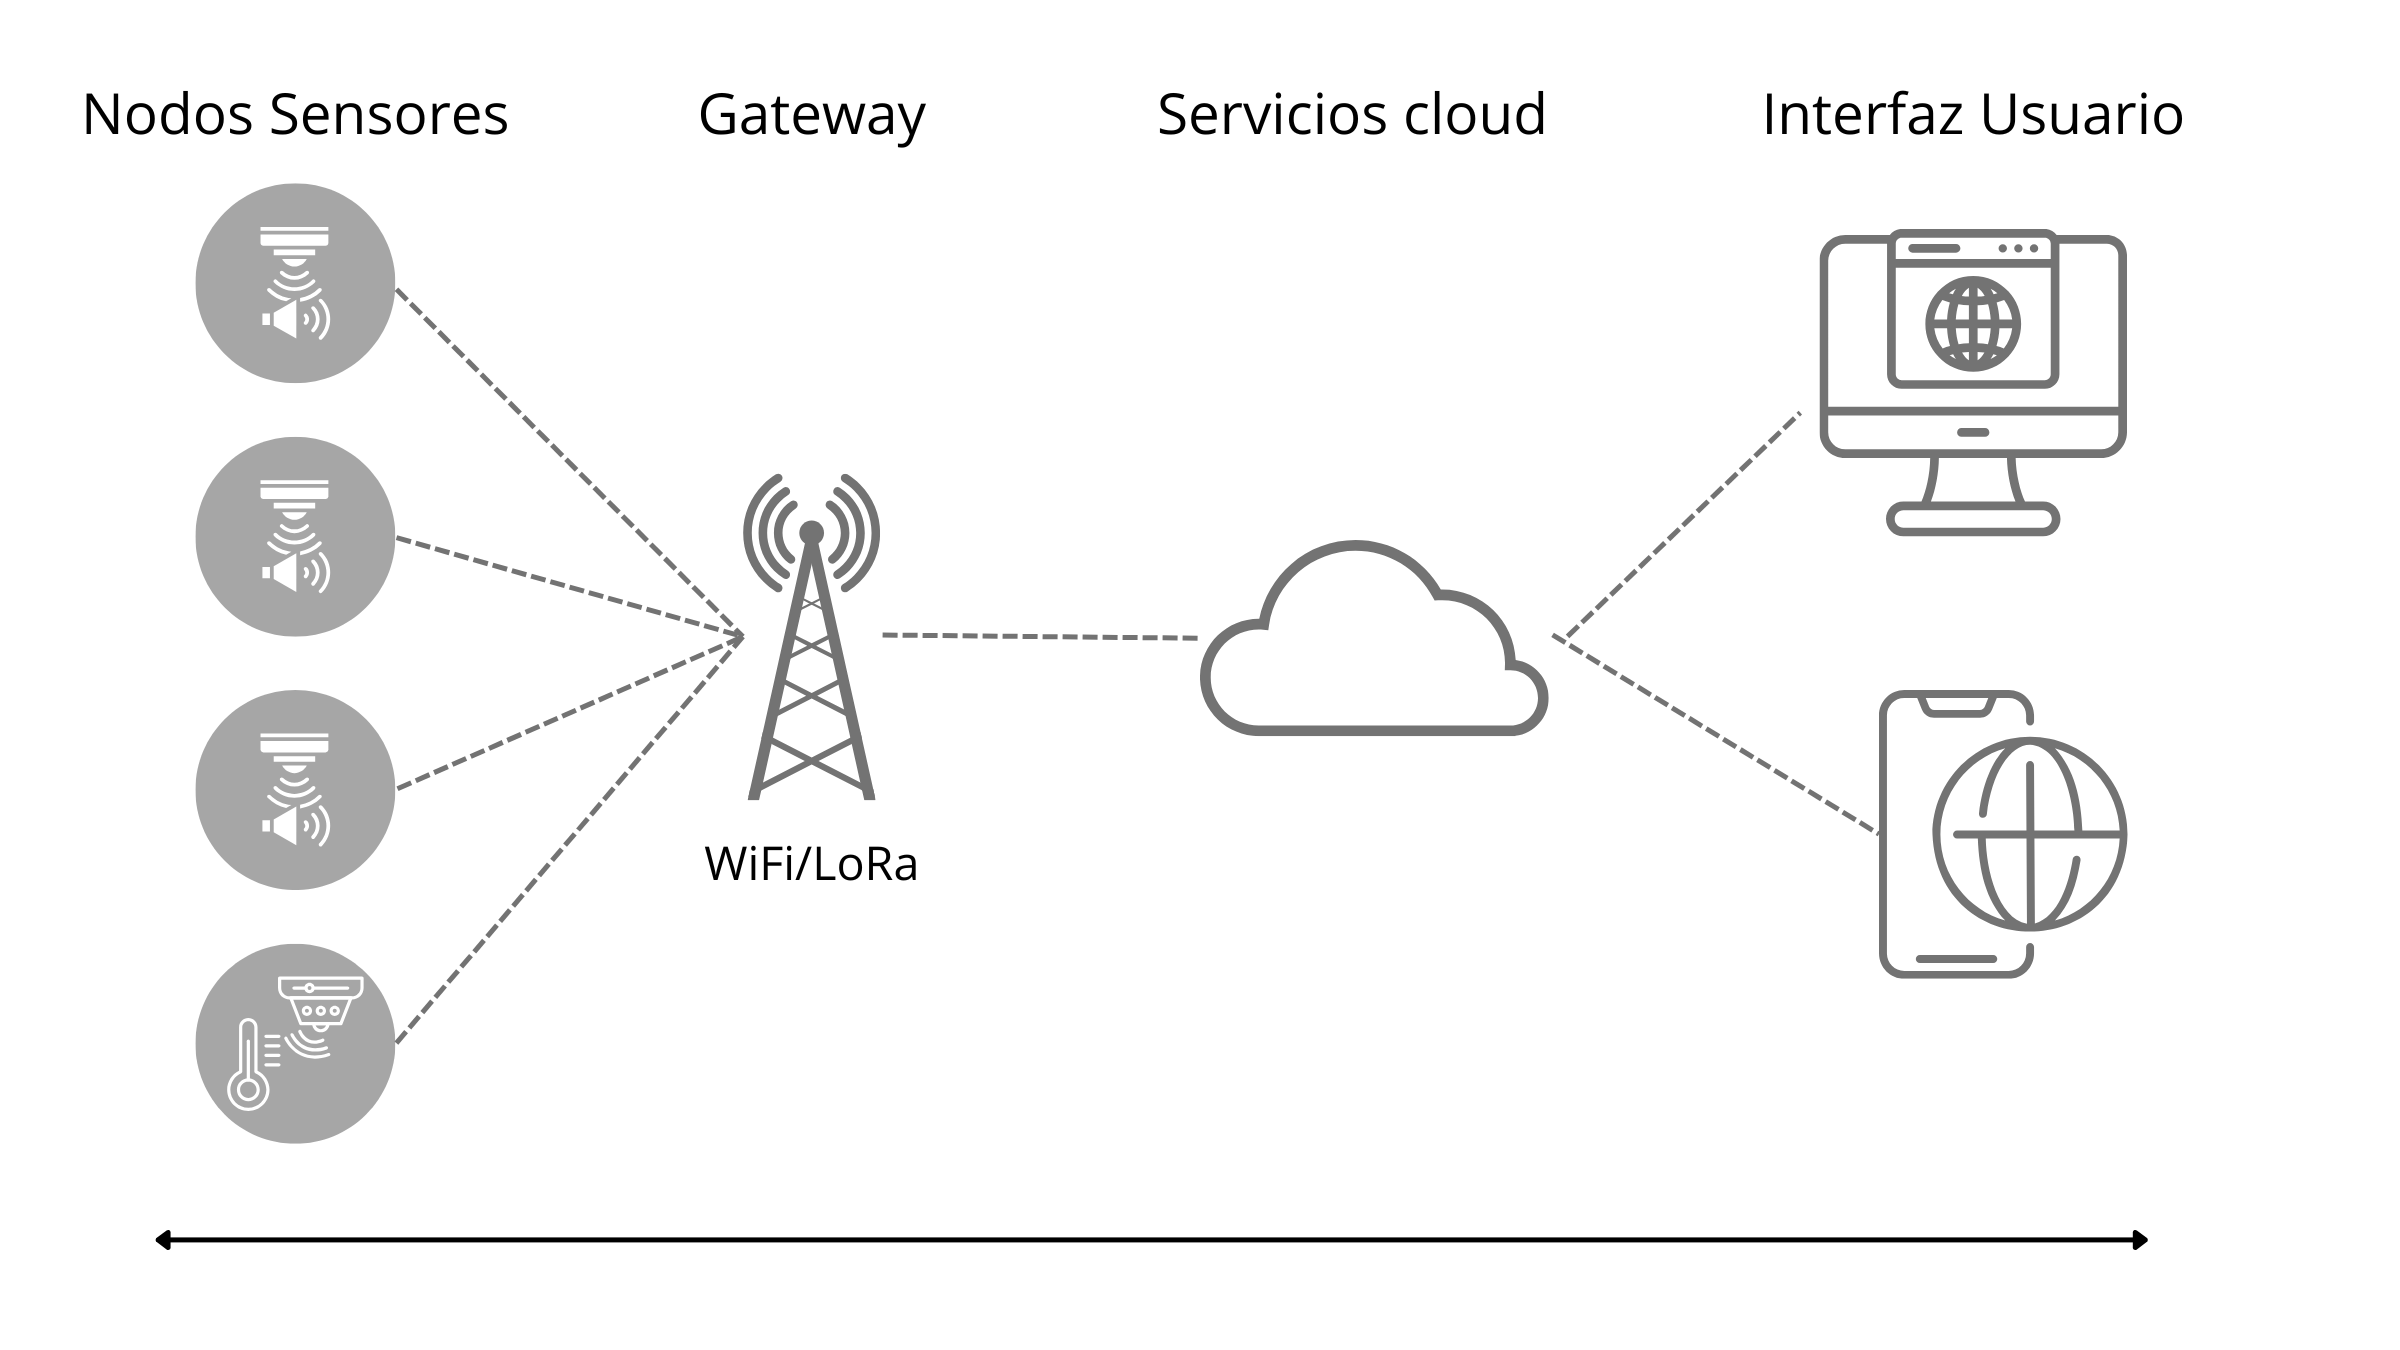
\includegraphics[width=.75\textwidth]{./Figuras/diagramaSist.png}
	\caption{Diagrama del sistema.}
	\label{fig:diagBloques}
	\end{figure}
	
	\vspace{25px}

\section{2. Identificación y análisis de los interesados}
\label{sec:interesados}



\begin{table}[ht]
%\caption{Identificación de los interesados}
%\label{tab:interesados}
\begin{tabularx}{\linewidth}{@{}|l|X|X|l|@{}}
\hline
\rowcolor[HTML]{C0C0C0} 
Rol           & Nombre y Apellido & Organización 	& Puesto 	\\ \hline
Cliente   & Ing. Mauricio Sejas Herbas       & Brazil Investment Hub        	& Gerente	\\ \hline
Responsable   & \authorname       & FIUBA        	& Alumno 	\\ \hline
Orientador    & \supname	      & \pertesupname 	& Director del Trabajo Final \\ \hline
Usuario final &  Gobiernos, alcaldias, empresas      &   Pública y privada     	&        -	\\ \hline
\end{tabularx}
\end{table}

• Orientador: el Mgtr. Rodolfo Raúl Terán Aiza cuenta con amplia experiencia en sistemas electromecánicos e instrumentación aplicada.


\section{3. Propósito del proyecto}
\label{sec:proposito}
 
Desarrollar un sistema IoT eficiente, escalable y de bajo costo para la medición y monitoreo en tiempo real de los niveles de 
ruido en entornos cerrados y pequeñas áreas urbanas que permita recopilar, procesar y visualizar datos acústicos de manera 
accesible. Capaz de proporcionar a los usuarios información precisa sobre la contaminación sonora en distintos espacios. 

\newpage

\section{4. Alcance del proyecto}
\label{sec:alcance}

La propuesta está orientada a ofrecer un sistema modular, escalable y de bajo consumo energético, con una infraestructura 
adaptable a distintos escenarios de uso.

El proyecto incluye:
\begin{itemize}
    \item \textbf{Diseño e implementación de un sistema IoT para monitoreo de ruido}, compuesto por nodos sensores, un módulo de comunicación y una plataforma en la nube.
    \begin{itemize}
        \item Desarrollo de un prototipo funcional con tres nodos sensores distribuidos en un entorno de prueba.
        \item Selección, calibración y configuración de sensores de ruido con un rango de medición entre 30 y 120 dB, 
        que garantice una precisión aceptable para el análisis acústico.
        \item Integración con microcontrolador esp32 que permita el procesamiento de datos en la transmisión de información.
        \item Implementación de un módulo de conectividad inalámbrica utilizando tecnologías Wi-Fi para entornos cerrados y LoRa para áreas urbanas con baja cobertura de red.
    \end{itemize}
    
    \item \textbf{Desarrollo de una plataforma en la nube para almacenamiento y visualización de datos.}
    \begin{itemize}
        \item Configuración de una base de datos para el almacenamiento de registros históricos y análisis posterior.
        \item Implementación de un \textit{dashboard} web accesible para la consulta de datos en tiempo real, que permita la visualización de mediciones y tendencias históricas.
        \item Incorporación de un sistema de alertas configurables para notificar a los usuarios cuando los niveles de ruido superen los umbrales predefinidos.
    \end{itemize}
    
    \item \textbf{Optimización energética del sistema}, asegurando bajo consumo y autonomía en los nodos sensores.
    \begin{itemize}
        \item Implementación de estrategias de bajo consumo en los microcontroladores, utilizando modos de suspensión y transmisión periódica.
        \item Evaluación del uso de baterías recargables con posibilidad de integración de paneles solares en escenarios de monitoreo prolongado.
    \end{itemize}
    
\end{itemize}

El presente proyecto no incluye:
\begin{itemize}
    \item Reducción o mitigación del ruido ambiental, ya que su enfoque se limita a la medición y análisis de los niveles de ruido.
    \item Integración con modelos de inteligencia artificial o análisis predictivo en esta fase inicial, aunque el sistema está diseñado para futuras ampliaciones en este sentido.
    \item Desarrollo de una aplicación móvil nativa; el acceso a los datos y la visualización del sistema se realizarán únicamente a través de una interfaz web.
    \item Implementación en escenarios reales fuera del alcance de pruebas controladas, limitándose en esta etapa a un entorno de prueba definido para la validación del prototipo.
\end{itemize}

\section{5. Supuestos del proyecto}
\label{sec:supuestos}

Para el desarrollo del presente proyecto se supone que:

\begin{itemize}
    \item No se considerarán regulaciones específicas sobre privacidad o normativas de manejo de datos, dado que el sistema solo recopilará información de niveles de ruido sin asociarlos a datos personales o identificables.
    \item Se asumirá que las condiciones de infraestructura en los entornos de prueba son representativas de espacios urbanos y cerrados típicos, sin interferencias extremas que afecten la captura y transmisión de datos.
    \item Se dispondrá de una red eléctrica estable en las áreas de prueba, que permita el funcionamiento de los sensores y la transmisión de datos sin interrupciones críticas.
    \item No se considerarán eventos extremos como fallos masivos de red, cortes prolongados de energía o interferencias radioeléctricas severas que puedan comprometer el funcionamiento del sistema.
    \item Se asumirá que las condiciones ambientales dentro de los entornos de prueba serán normales, sin presencia de factores climáticos extremos que puedan afectar la medición del sonido o el funcionamiento de los dispositivos.
    \item Se trabajará con un conjunto limitado de nodos sensores, sin escalabilidad masiva en esta fase del proyecto.
    \item No se contemplará la implementación de sistemas de redundancia avanzada para la transmisión y almacenamiento de datos, ya que el proyecto busca validar la funcionalidad básica del sistema en su fase inicial.
\end{itemize}


\section{6. Requerimientos}
\label{sec:requerimientos}

A continuación, se enumeran los requerimientos del sistema propuesto.

\begin{enumerate}
    \item \textbf{Requerimientos funcionales (prioridad alta):}
    \begin{enumerate}
        \item El sistema debe medir niveles de ruido ambiental en tiempo real con una frecuencia configurable (mínimo una medición cada 5 minutos).
        \item Los sensores deben registrar valores en dB con un rango de 30–120 dB y precisión máxima de ±2 dB.
        \item El microcontrolador debe procesar localmente los datos y transmitirlos a la nube a través de Wi-Fi o LoRaWan, según el entorno.
        \item El sistema debe generar una alerta automática cuando el nivel de ruido supere un umbral configurable.
        \item El sistema debe permitir almacenar los datos de manera estructurada y persistente en una base de datos alojada en un servidor remoto.
        \item El usuario debe poder acceder a los datos mediante un \textit{dashboard} web desde cualquier navegador moderno.
        \item El sistema debe estar probado en un entorno controlado como prueba de concepto, con documentación del despliegue y resultados.
    \end{enumerate}

    \item \textbf{Requerimientos de interfaz (prioridad alta):}
    \begin{enumerate}
        \item El usuario debe poder acceder a un \textit{dashboard} web desde navegadores modernos sin necesidad de instalar software adicional.
        \item La interfaz debe mostrar los niveles de ruido actuales, valores históricos y tendencias de forma visual y comprensible (por ejemplo, gráficos de líneas, colores de alerta, etc.).
        \item El usuario debe poder configurar el umbral de alertas desde la misma interfaz.
    \end{enumerate}

    \item \textbf{Requerimientos de hardware (prioridad alta):}
    \begin{enumerate}
        \item Cada nodo debe operar al menos 5 días seguidos con batería sin recarga (con opción de carga solar).
        \item Los sensores deben ser fácilmente reemplazables o reubicables.
        \item El sistema debe funcionar en ambientes interiores y exteriores moderadamente protegidos.
    \end{enumerate}

    \item \textbf{Requerimientos de \textit{backend} y almacenamiento (prioridad alta):}
    \begin{enumerate}
        \item La base de datos utilizada deberá permitir el almacenamiento estructurado de registros históricos con acceso rápido (PostgreSQL o SQLite en entorno cloud).
    \end{enumerate}

    \item \textbf{Requerimientos de interoperabilidad (prioridad baja, opcional):}
    \begin{enumerate}
        \item El sistema podrá exportar los datos en formato CSV o JSON para análisis externo (requerimiento opcional).
    \end{enumerate}

    \item \textbf{Requerimientos de seguridad (prioridad media):}
    \begin{enumerate}
        \item El acceso al \textit{dashboard} debe estar protegido mediante credenciales de usuario.
        \item El \textit{backend} debe implementar un sistema básico de autenticación, como JWT o similar, para proteger las rutas de acceso a datos.
        \item Las comunicaciones entre el nodo y el servidor deben utilizar protocolos seguros, salvo en casos justificados por limitaciones técnicas.
    \end{enumerate}

    \item \textbf{Requerimientos normativos (prioridad alta):}
    \begin{enumerate}
        \item El sistema debe contemplar los valores límite de exposición al ruido establecidos por la Ley N.º 1540 de la Ciudad Autónoma de Buenos Aires.
        \item Las alertas deberán configurarse con base en dichos umbrales: 55 dB para interiores diurnos, 45 dB para nocturnos, 70 dB en espacios públicos al aire libre.
    \end{enumerate}


    \item \textbf{Requerimientos de documentación (prioridad alta):}
    \begin{enumerate}
        \item Se debe desarrollar una memoria descriptiva del sistema, incluyendo el hardware, software y configuración utilizada.
        \item Se debe incluir un manual de usuario y un manual de instalación y configuración. 
        \item La documentación debe contemplar información de APIs desarrolladas para la comunicación. 
    \end{enumerate}

\end{enumerate}




\section{7. Historias de usuarios (\textit{Product backlog})}
\label{sec:backlog}

\section{Historias de Usuario}

\begin{enumerate}
    \item \textbf{Como administrador del sistema quiero visualizar en un panel web los niveles actuales de ruido en tiempo real para monitorear el estado acústico del entorno.}

    \textit{Story points}: 8 (complejidad: 3, dificultad: 2, incertidumbre: 2)

    \textbf{Criterios de aceptación}:
    \begin{itemize}
        \item El \textit{dashboard} debe mostrar los valores actuales de dB por nodo sensor.
        \item La información debe actualizarse automáticamente cada 5 minutos o menos.
        \item El diseño debe ser claro, responsivo y accesible desde cualquier navegador moderno.
    \end{itemize}

    \item \textbf{Como usuario del sistema quiero recibir una alerta cuando el nivel de ruido supere un umbral definido para poder tomar acciones correctivas.}

    \textit{Story points}: 8 (complejidad: 2, dificultad: 2, incertidumbre: 2)

    \textbf{Criterios de aceptación}:
    \begin{itemize}
        \item El usuario podrá configurar el umbral desde el \textit{dashboard}.
        \item El sistema debe generar la alerta a partir de la configuración de umbrales del usuario.
        \item La alerta se despliega en el aplicativo web y notifica al usuario.
    \end{itemize}

    \item \textbf{Como dadministrador quiero que los datos de ruido se almacenen automáticamente en una base de datos en la nube para garantizar persistencia y análisis posterior.}

    \textit{Story points}: 8 (complejidad: 3, dificultad: 3, incertidumbre: 2)

    \textbf{Criterios de aceptación}:
    \begin{itemize}
        \item Cada medición debe almacenarse con marca de tiempo y origen del sensor.
        \item El sistema debe guardar al menos 7 días consecutivos de datos históricos.
        \item La base de datos debe ser accesible desde el \textit{backend} de forma eficiente.
    \end{itemize}

    \item \textbf{Como administrador del sistema quiero poder exportar los datos en formato CSV o JSON para su uso en otros análisis.}

    \textit{Story points}: 5 (complejidad: 2, dificultad: 1, incertidumbre: 2)

    \textbf{Criterios de aceptación}:
    \begin{itemize}
        \item El \textit{dashboard} debe tener un botón de exportación por rango de fechas.
        \item El archivo generado debe contener datos válidos y bien estructurados.
        \item Debe ser posible descargarlo desde cualquier navegador.
    \end{itemize}

    \item \textbf{Como usuario quiero poder iniciar sesión con credenciales para acceder de forma segura al sistema.}

    \textit{Story points}: 8 (complejidad: 2, dificultad: 2, incertidumbre: 2)

    \textbf{Criterios de aceptación}:
    \begin{itemize}
        \item Debe existir una pantalla de \textit{login} con usuario y contraseña.
        \item Las credenciales deben verificarse en el \textit{backend} con JWT u otra solución segura.
        \item No se debe acceder al \textit{dashboard} sin estar autenticado.
    \end{itemize}

    \item \textbf{Como administrador quiero poder ver el estado de los nodos sensores para verificar que estén funcionando correctamente.}

    \textit{Story points}: 8 (complejidad: 3, dificultad: 2, incertidumbre: 2)

    \textbf{Criterios de aceptación}:
    \begin{itemize}
        \item El sistema debe mostrar el estado de conexión de cada nodo (activo/inactivo).
        \item Cada nodo debe tener un identificador único.
        \item El \textit{dashboard} debe mostrar su ubicación aproximada o nombre de ubicación.
    \end{itemize}

    \item \textbf{Como técnico de campo quiero desplegar un nodo sensor y que este se conecte automáticamente al sistema para facilitar su instalación.}

    \textit{Story points}: 8 (complejidad: 2, dificultad: 2, incertidumbre: 2)

    \textbf{Criterios de aceptación}:
    \begin{itemize}
        \item El nodo debe autoconectarse a la red y al \textit{backend} al encenderse.
        \item El nodo debe enviar una primera medición para confirmar su activación.
        \item El proceso no debe requerir configuración manual avanzada.
    \end{itemize}
\end{enumerate}

\section{8. Entregables principales del proyecto}
\label{sec:entregables}

A continuación, se enumeran los entregables que serán producidos como resultado del desarrollo del proyecto. 

\begin{itemize}
    \item Prototipo físico funcional del sistema IoT con al menos tres nodos sensores de ruido operativos.
    \item Código fuente del \textit{firmware} para los microcontroladores, con comentarios y estructura comprensible.
    \item \textit{backend} del sistema implementado en entorno cloud con endpoints documentados.
    \item \textit{Dashboard} web funcional para la visualización de datos, alertas e historial de mediciones.
    \item Base de datos implementada y operativa, con estructura simple y datos históricos registrados durante las pruebas.
    \item Diagrama de bloques del sistema.
    \item Esquema básico de conexiones electrónicas.
    \item Manual de instalación y uso
    \item Memoria del trabajo final.
    
\end{itemize}



\section{9. Desglose del trabajo en tareas}
\label{sec:wbs}

\section{Desglose del trabajo en tareas}

A continuación, se presenta el desglose del trabajo en tareas (WBS) del proyecto, con estimación de horas por grupo y su vinculación directa con las historias de usuario (HU) definidas.

\begin{enumerate}
    \item Planificación y diseño del sistema (60 h)
    \begin{enumerate}
        \item Análisis detallado de requerimientos y casos de uso (10 h) 
        \item Diseño del sistema y definición de arquitectura general (16 h) 
        \item Selección de sensores y componentes electrónicos (13 h) 
        \item Diseño del diagrama de bloques del sistema (6 h) 
        \item Definición de estructura de base de datos y \textit{backend} (15 h) 
    \end{enumerate}

    \item Desarrollo del \textit{firmware} para nodos sensores (120 h)
    \begin{enumerate}
        \item Configuración e integración de sensores de ruido con microcontrolador (25 h) 
        \item Programación del procesamiento de señales de medición en dB (30 h)
        \item Implementación de modos de bajo consumo  \textit{deep sleep} (15 h) 
        \item Transmisión de datos vía Wi-Fi y LoRa (30 h) 
        \item Calibración básica con sonómetro de referencia (8 h) 
        \item Documentación técnica del \textit{firmware} (12 h) 
    \end{enumerate}

    \item \textit{backend} y almacenamiento de datos (110 h)
    \begin{enumerate}
        \item Configuración de base de datos (PostgreSQL) (15 h) 
        \item Implementación del \textit{backend} en servidor cloud (30 h) 
        \item Desarrollo de API para recepción y consulta de datos (25 h) 
        \item Gestión de usuarios y autenticación (JWT) (15 h) 
        \item Pruebas de integración y validación (10 h)
        \item Documentación técnica del \textit{backend} (15 h) 
    \end{enumerate}

    \item Desarrollo del \textit{dashboard} web (115 h)
    \begin{enumerate}
        \item Maquetado del \textit{dashboard} e interfaz responsiva (15 h) 
        \item Visualización de niveles de ruido (15 h) 
        \item Indicadores visuales (15 h) 
        \item Configuración de umbrales de alerta por el usuario (25 h) 
        \item Función de exportación de datos (CSV/JSON) (10 h) 
        \item Implementación de login y control de acceso (20 h) 
        \item Pruebas funcionales y correcciones (7 h) 
        \item Documentación técnica del \textit{frontend} (8 h) 
    \end{enumerate}

    \item Despliegue del prototipo y validación (65 h)
    \begin{enumerate}
        \item Montaje y prueba de nodos sensores en entorno de prueba (15 h) 
        \item Monitoreo del sistema en operación (20 h) 
        \item Análisis de resultados y comportamiento (15 h) 
        \item Documentación de la prueba de concepto (15 h) 
    \end{enumerate}

    \item Documentación y entregables (150 h)
    \begin{enumerate}
        \item Redacción de la memoria del proyecto (70 h) 
        \item Elaboración del manual de usuario (20 h) 
        \item Preparación de presentación final (20 h) 
        \item Revisión de redacción, corrección y estilo (10 h) 
        \item Diagramas (bloques, instalación, conexiones, Gantt) (20 h) 
        \item Organización de anexos y referencias (10 h) 
    \end{enumerate}
\end{enumerate}

\textbf{Cantidad total de horas: 620 h}

\newpage
\section{10. Diagrama de Activity On Node}
\label{sec:AoN}

\begin{figure}[htpb]
\centering 
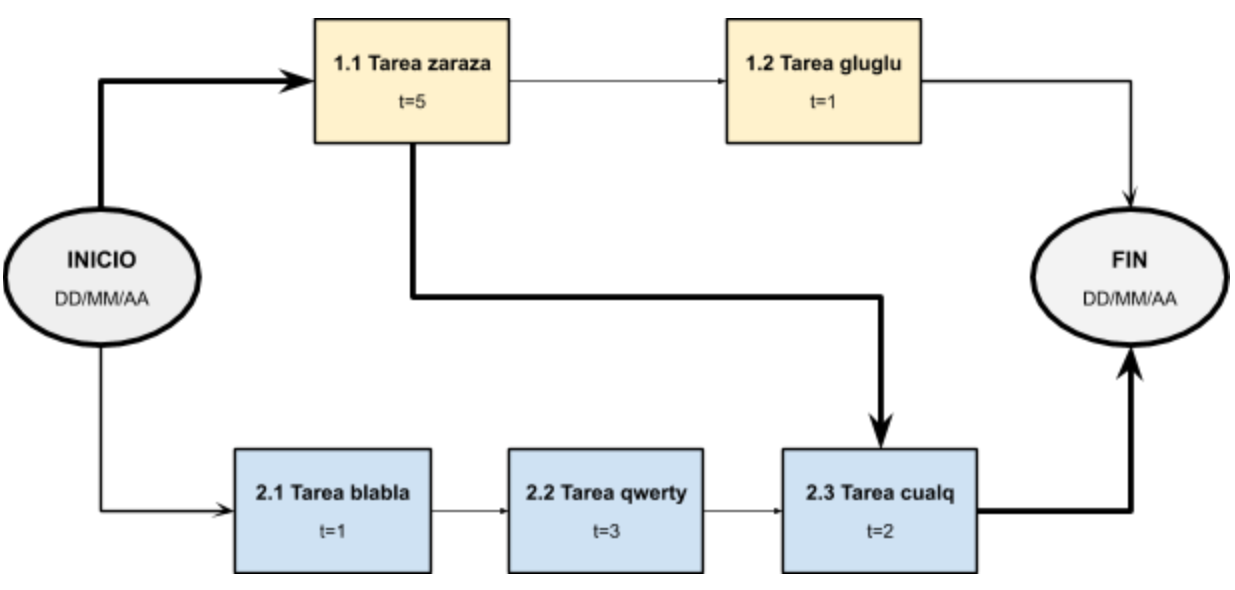
\includegraphics[width=1.05\textwidth]{./Figuras/AoN.png}
\caption{Diagrama de \textit{Activity on Node}.}
\label{fig:AoN}
\end{figure}
\begin{itemize}
    \item Las líneas más gruesas de color rojo representan la ruta crítica del proyecto.
    \item Las duraciones de las tareas están expresadas en horas.
\end{itemize}


\newpage

\section{11. Diagrama de Gantt}
\label{sec:gantt}
En la figura \ref{fig:AoN1} se muestra el diagrama de Gantt a nivel general del proyecto.
\begin{figure}[htpb]
    \centering 
    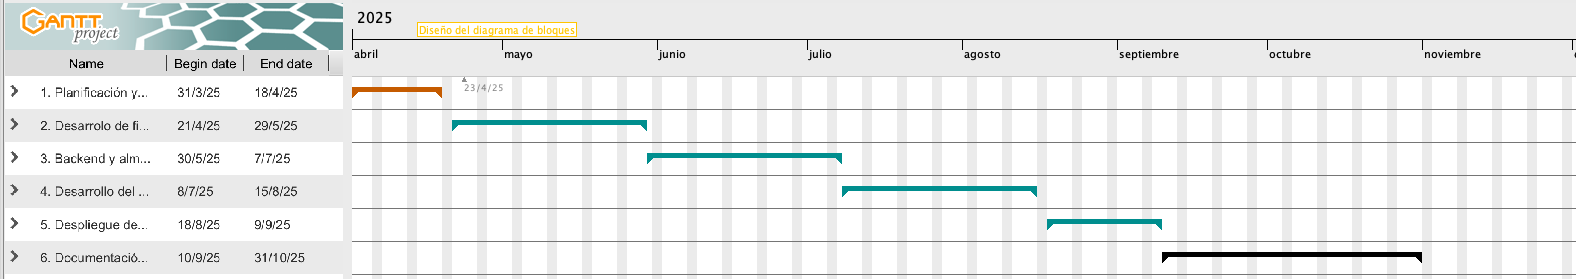
\includegraphics[width=1.05\textwidth]{./Figuras/gantt1.png}
    \caption{Diagrama de Gantt a nivel general del proyecto.}
    \label{fig:AoN1}
    \end{figure}


En la figura \ref{fig:AoN2} se muestra el diagrama de Gantt para la planificación y diseño del sistema.
\begin{figure}[htpb]
    \centering 
    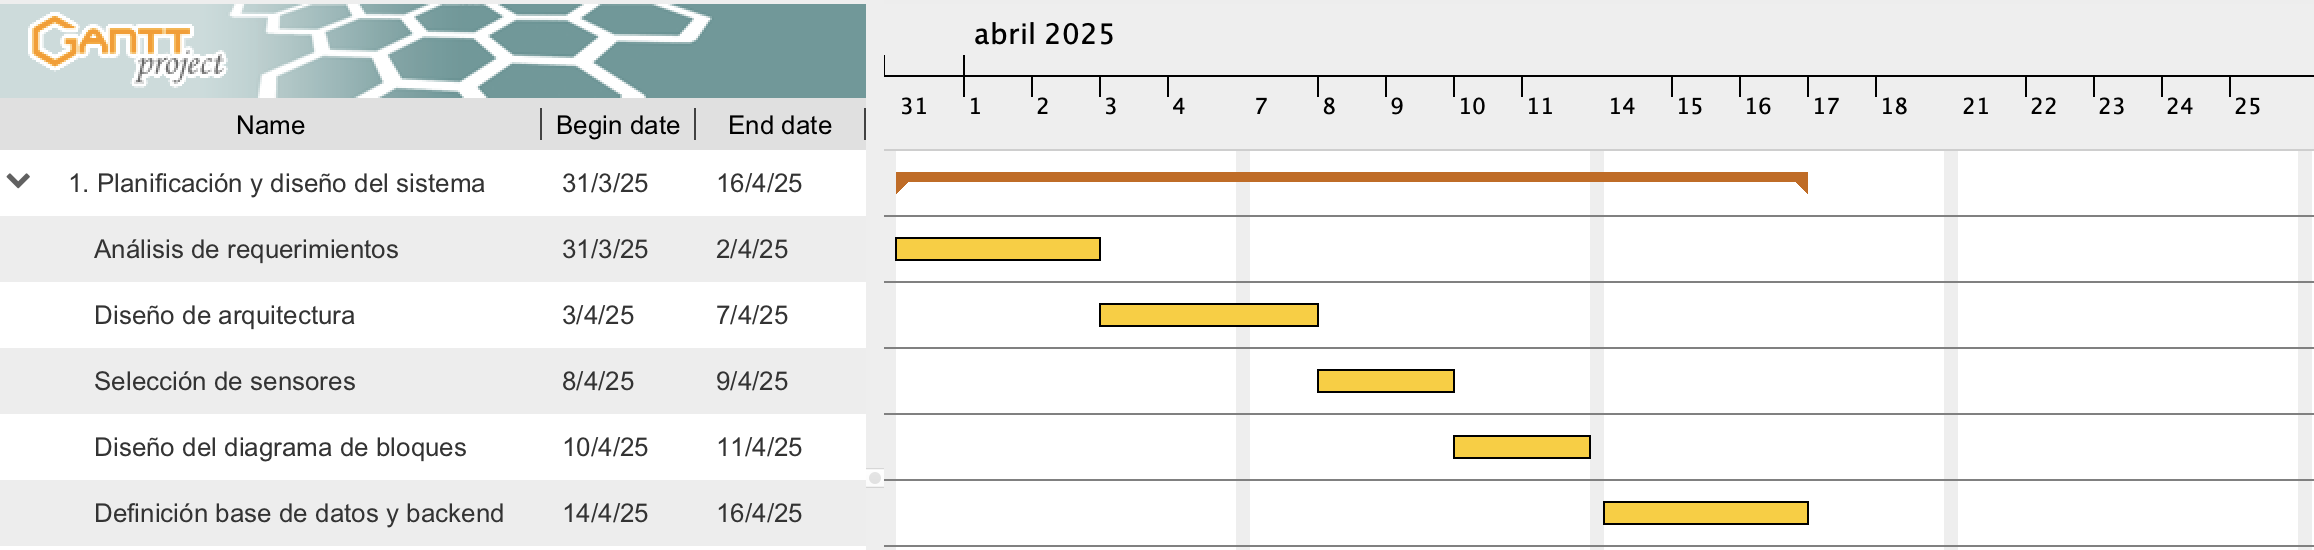
\includegraphics[width=1.05\textwidth]{./Figuras/gantt2.png}
    \caption{Diagrama de Gantt etapa 1.}
    \label{fig:AoN2}
    \end{figure}

En la figura \ref{fig:AoN3} se muestra el diagrama de Gantt para el desarrollo del \textit{firmware} para nodos sensores.
\begin{figure}[htpb]
    \centering 
    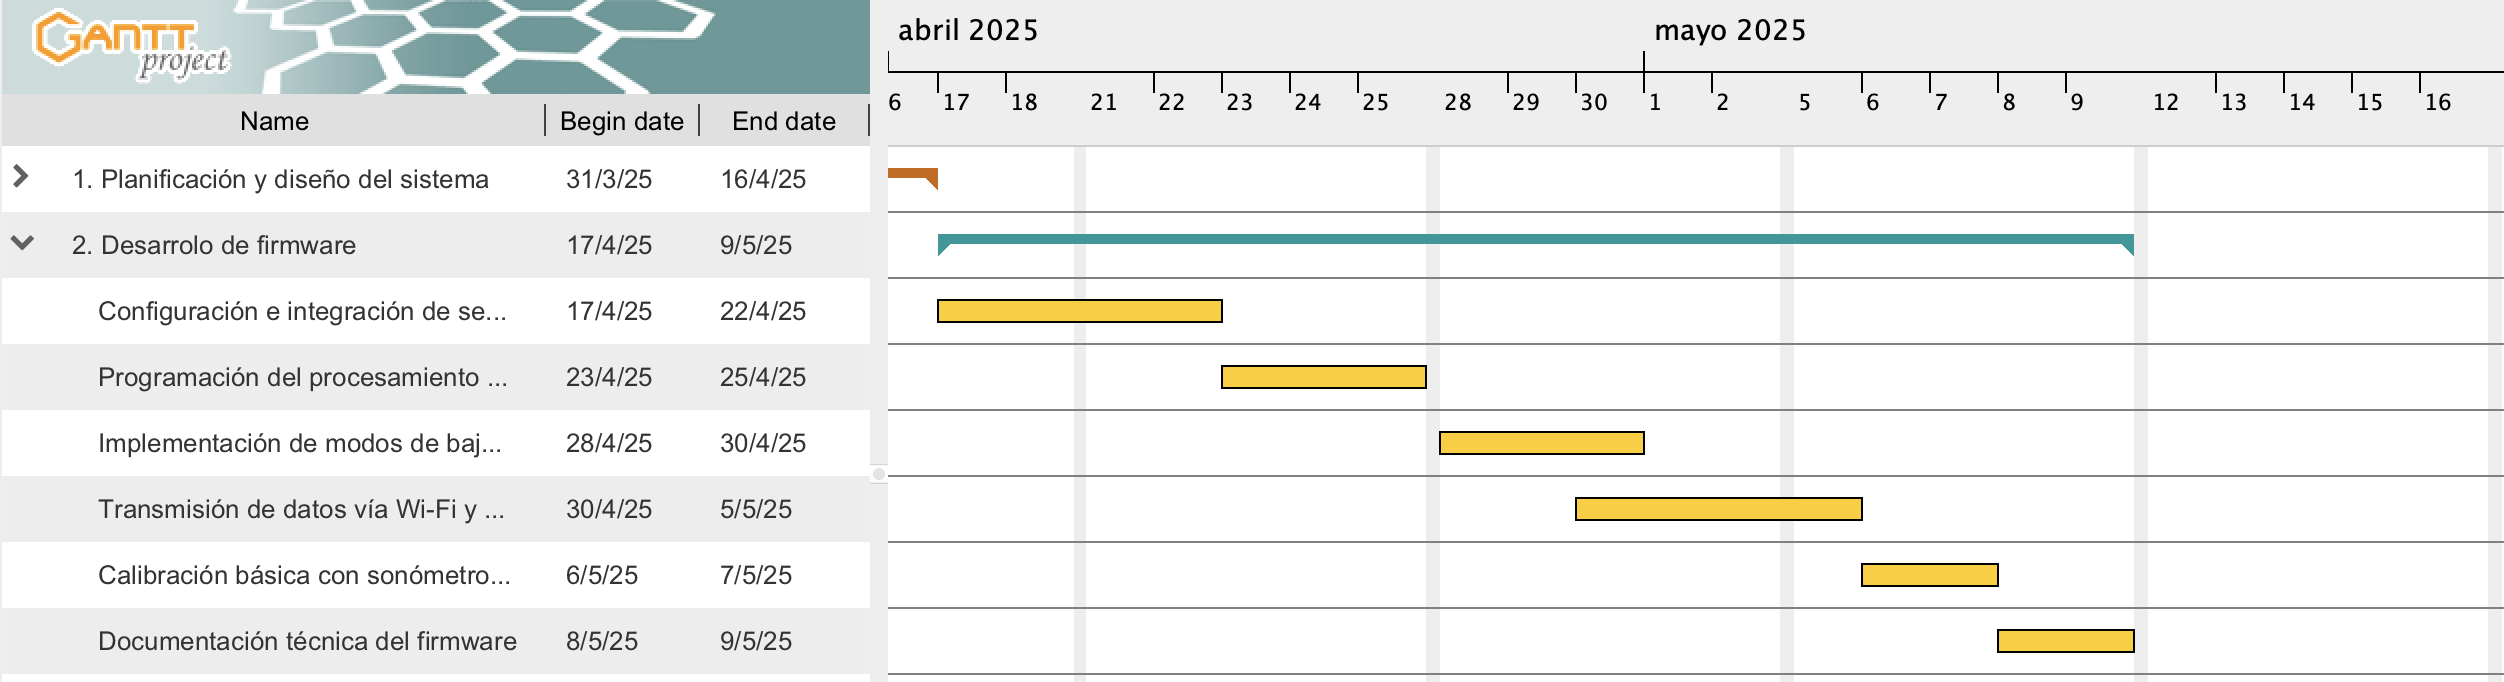
\includegraphics[width=1.05\textwidth]{./Figuras/gantt3.png}
    \caption{Diagrama de Gantt etapa 2.}
    \label{fig:AoN3}
    \end{figure}

    \newpage

En la figura \ref{fig:AoN4} se muestra el diagrama de Gantt para el desarrollo de \textit{backend} y almacenamiento de datos.
\begin{figure}[htpb]
    \centering 
    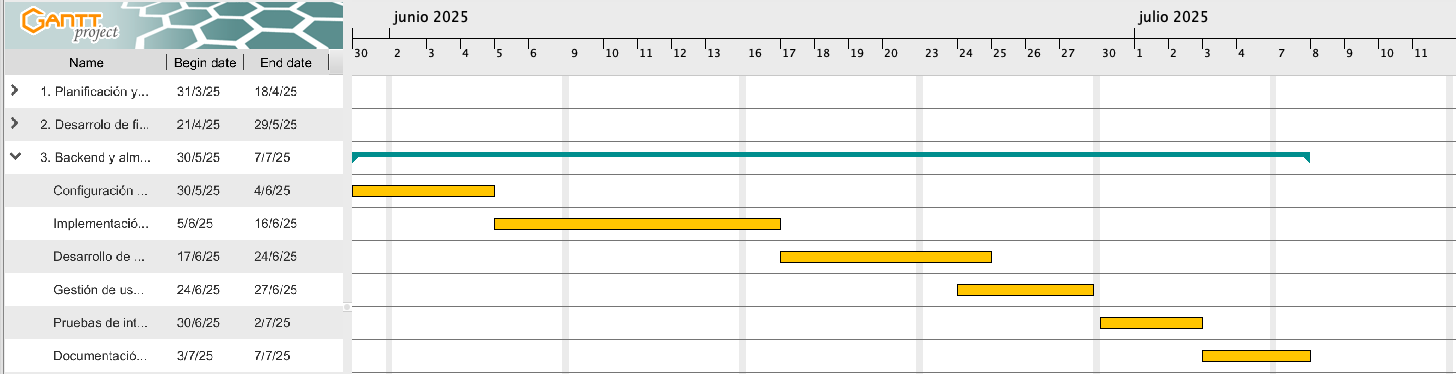
\includegraphics[width=1.05\textwidth]{./Figuras/gantt4.png}
    \caption{Diagrama de Gantt etapa 3.}
    \label{fig:AoN4}
    \end{figure}

En la figura \ref{fig:AoN5} se muestra el diagrama de Gantt para el desarrollo del Desarrollo del \textit{dashboard} web.
\begin{figure}[htpb]
    \centering 
    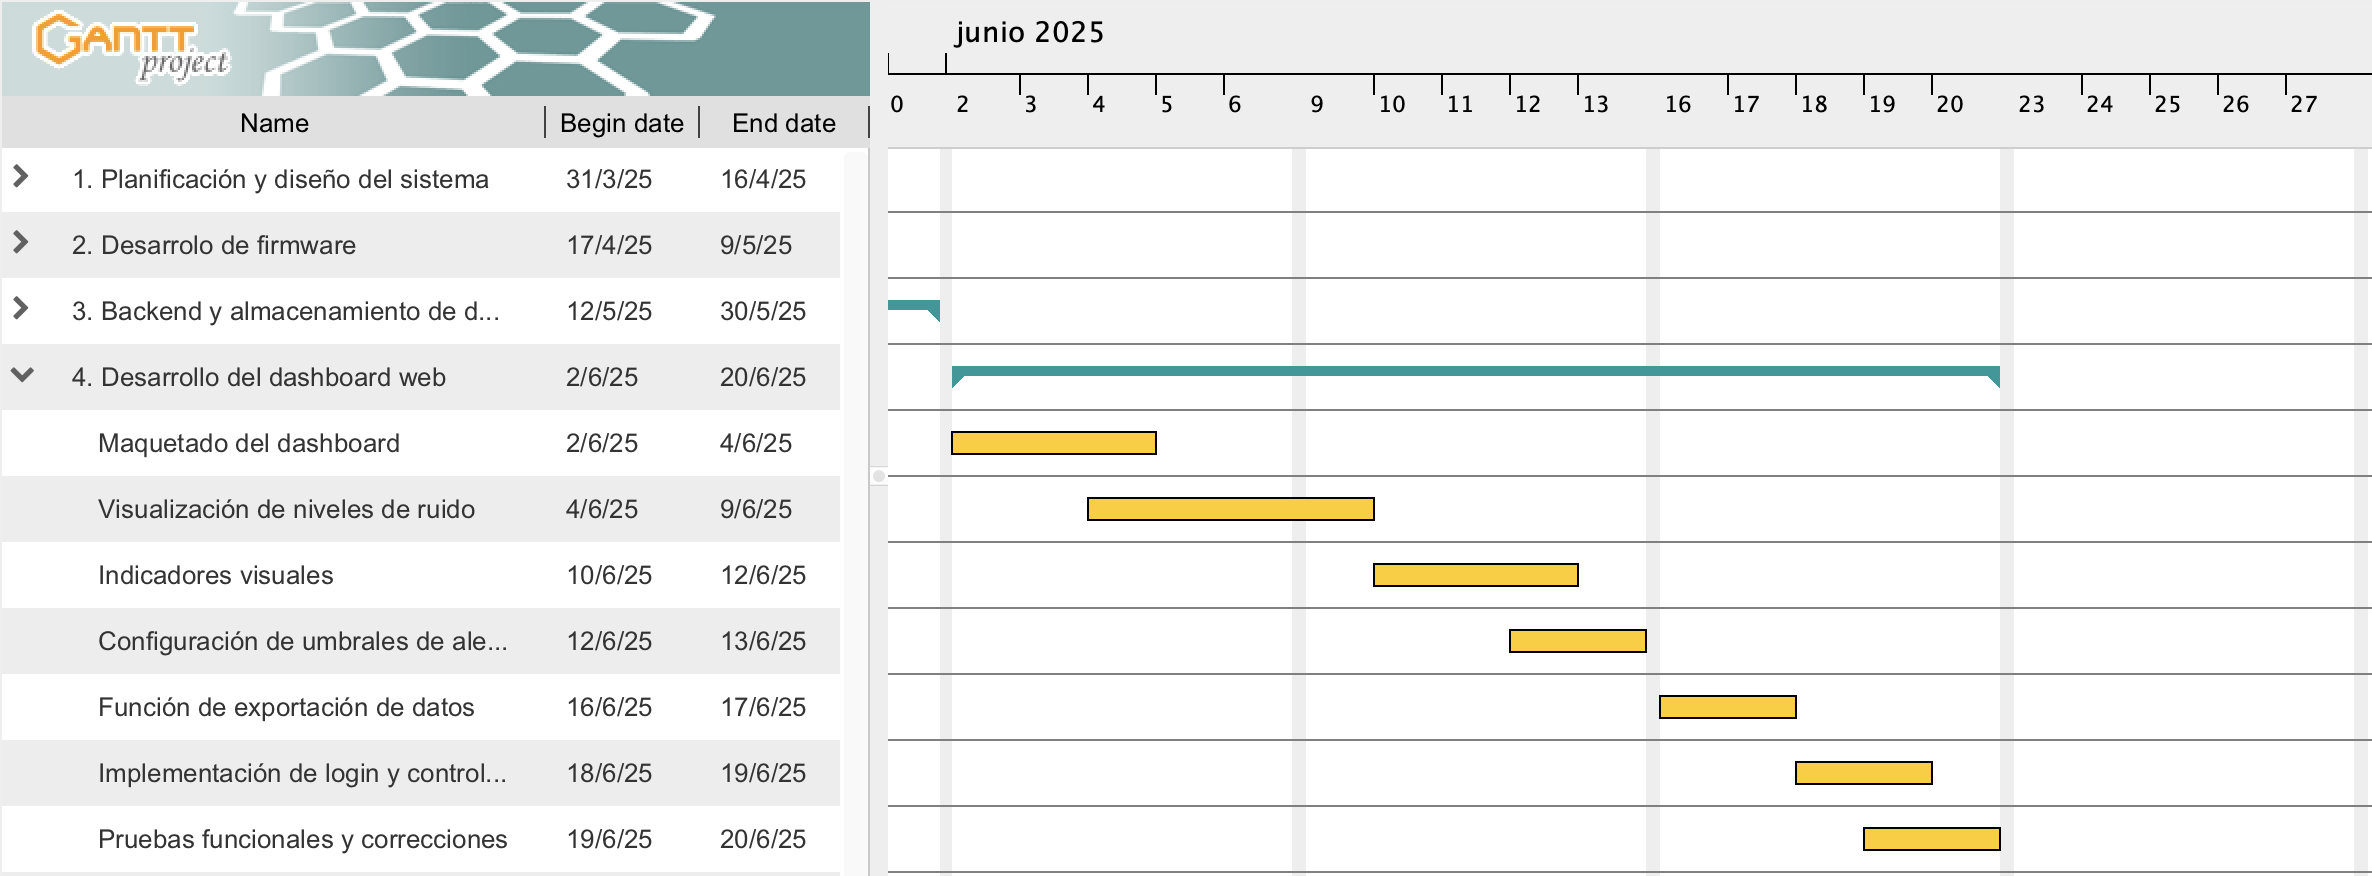
\includegraphics[width=1.05\textwidth]{./Figuras/gantt5.png}
    \caption{Diagrama de Gantt etapa 4.}
    \label{fig:AoN5}
    \end{figure}

    \newpage

En la figura \ref{fig:AoN6} se muestra el diagrama de Gantt para el despliegue del prototipo y validación.
\begin{figure}[htpb]
    \centering 
    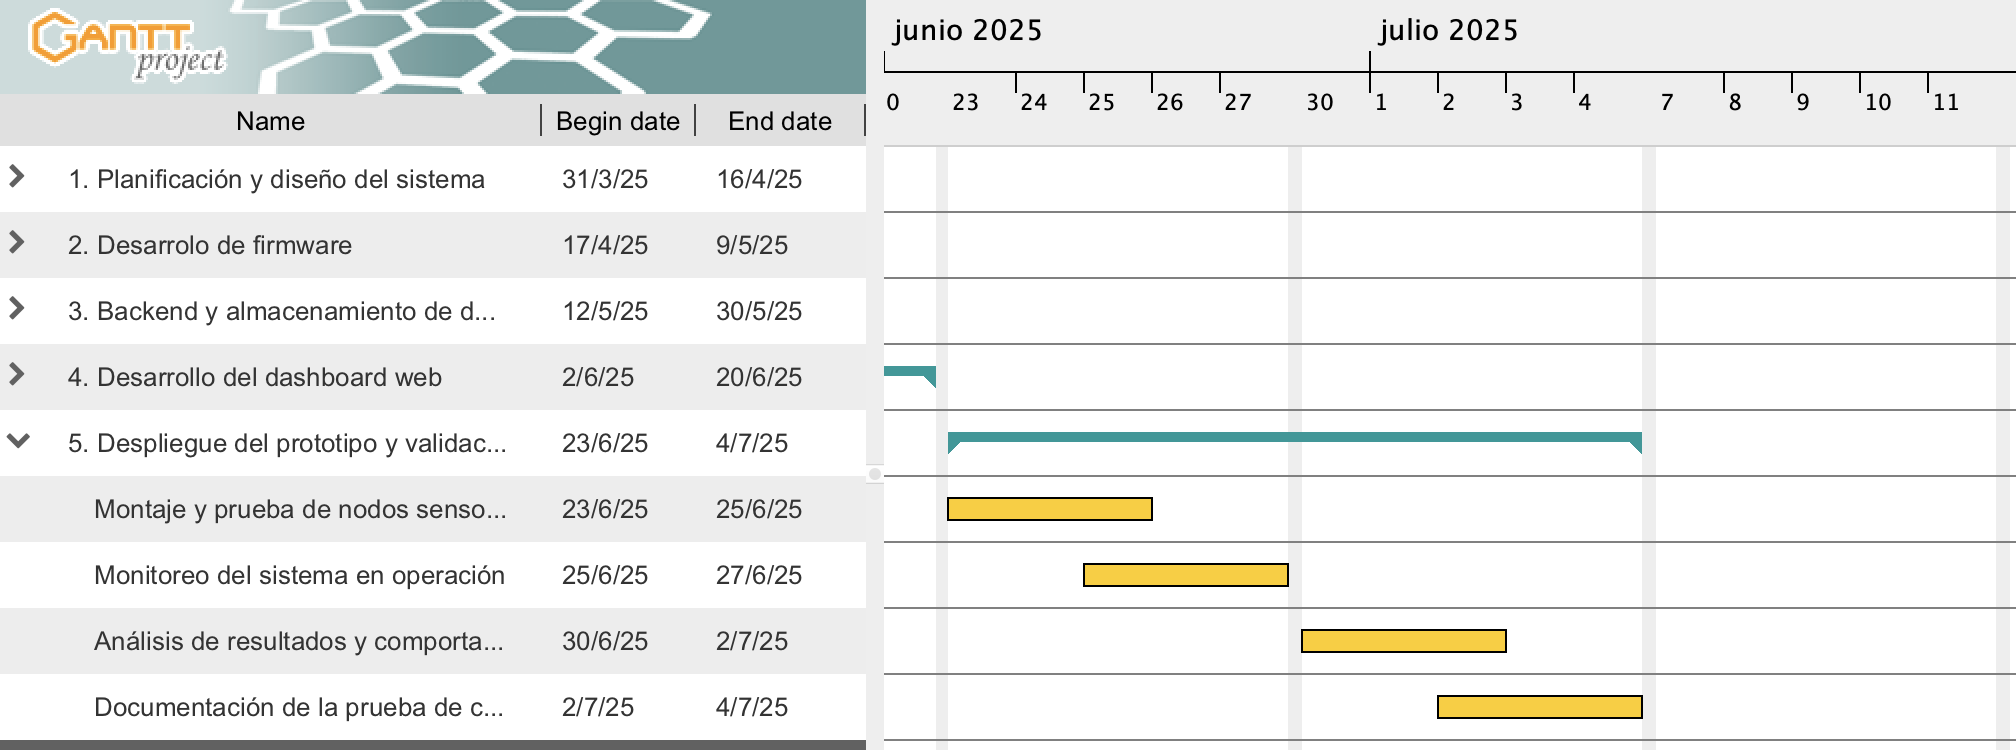
\includegraphics[width=1.05\textwidth]{./Figuras/gantt6.png}
    \caption{Diagrama de Gantt etapa 5.}
    \label{fig:AoN6}
    \end{figure}

En la figura \ref{fig:AoN7} se muestra el diagrama de Gantt para el desarrollo de la documentación y entregables.
\begin{figure}[htpb]
    \centering 
    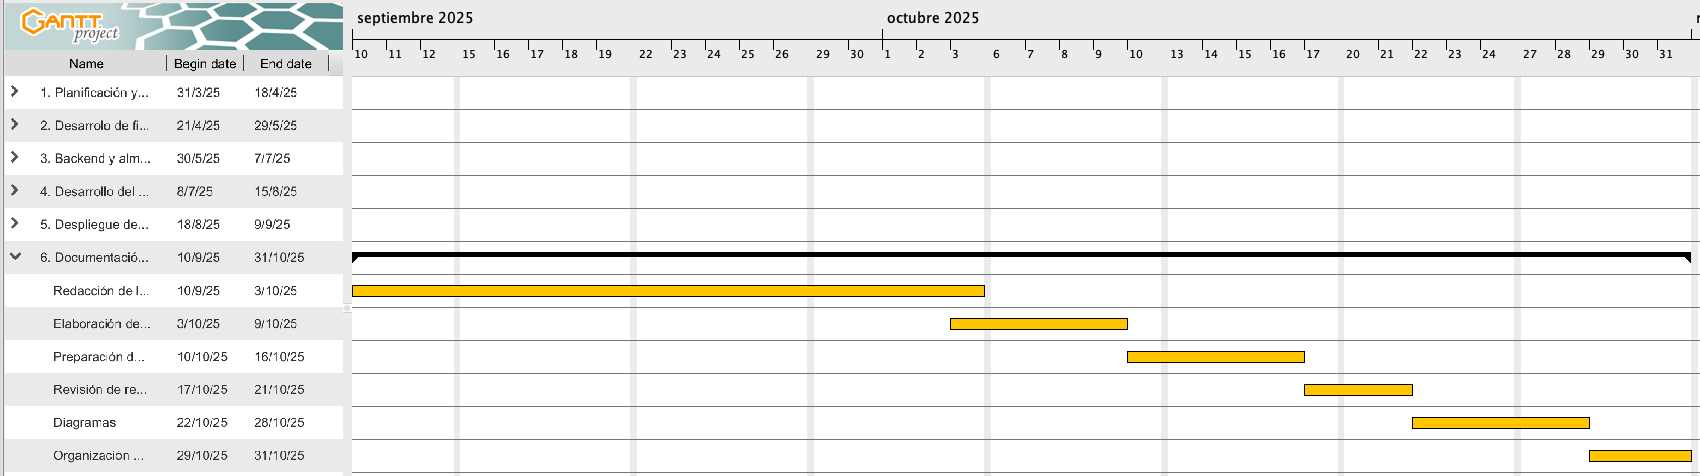
\includegraphics[width=1.05\textwidth]{./Figuras/gantt7.png}
    \caption{Diagrama de Gantt etapa 6.}
    \label{fig:AoN7}
    \end{figure}


\newpage

\section{12. Presupuesto detallado del proyecto}
\label{sec:presupuesto}
Los valores están expresados en pesos argentinos (ARS), cotización abril 2025.

\begin{table}[htpb]
\centering
\begin{tabularx}{\linewidth}{@{}|X|c|r|r|@{}}
\hline
\rowcolor[HTML]{C0C0C0} 
\multicolumn{4}{|c|}{\cellcolor[HTML]{C0C0C0}COSTOS DIRECTOS} \\ \hline
\rowcolor[HTML]{C0C0C0} 
Descripción &
  \multicolumn{1}{c|}{\cellcolor[HTML]{C0C0C0}Cantidad} &
  \multicolumn{1}{c|}{\cellcolor[HTML]{C0C0C0}Valor unitario} &
  \multicolumn{1}{c|}{\cellcolor[HTML]{C0C0C0}Valor total} \\ \hline
  Sensores de ruido (micrófono electret + módulo amplificador)&
  \multicolumn{1}{c|}{3} &
  \multicolumn{1}{c|}{ARS 8.000} &
  \multicolumn{1}{c|}{ARS 24.000} \\ \hline
 ESP32 con LoRa&
  \multicolumn{1}{c|}{3} &
  \multicolumn{1}{c|}{ARS 17.000} &
  \multicolumn{1}{c|}{ARS 51.000} \\ \hline
  Caja protectora para cada nodo&
  \multicolumn{1}{c|}{3} &
  \multicolumn{1}{c|}{ARS 10.000} &
  \multicolumn{1}{c|}{ARS 30.000} \\ \hline
  Base de datos PostgreSQL (uso limitado - estimado equivalente)&
  \multicolumn{1}{c|}{1} &
  \multicolumn{1}{c|}{ARS 2.000} &
  \multicolumn{1}{c|}{ARS 2.000} \\ \hline
  Sensor de temperatura/humedad para compensación acústica (DHT22)&
  \multicolumn{1}{c|}{1} &
  \multicolumn{1}{c|}{ARS 12.000} &
  \multicolumn{1}{c|}{ARS 12.000} \\ \hline
  Gateway LoRa (alternativa: WisGate Edge Lite 2)&
  \multicolumn{1}{c|}{1} &
  \multicolumn{1}{c|}{ARS 85.000} &
  \multicolumn{1}{c|}{ARS 85.000} \\ \hline
  Componentes electrónicos varios (resistencias, jumpers, protoboards)&
  \multicolumn{1}{c|}{1} &
  \multicolumn{1}{c|}{ARS 10.000} &
  \multicolumn{1}{c|}{ARS 10.000} \\ \hline
  Horas de trabajo&
  \multicolumn{1}{c|}{620} &
  \multicolumn{1}{c|}{ARS 10.000} &
  \multicolumn{1}{c|}{ARS 6.200.000} \\ \hline

\multicolumn{3}{|c|}{SUBTOTAL} &
  \multicolumn{1}{c|}{ARS 6.414.000} \\ \hline
\rowcolor[HTML]{C0C0C0} 
\multicolumn{4}{|c|}{\cellcolor[HTML]{C0C0C0}COSTOS INDIRECTOS} \\ \hline
\rowcolor[HTML]{C0C0C0} 
Descripción &
  \multicolumn{1}{c|}{\cellcolor[HTML]{C0C0C0}Cantidad} &
  \multicolumn{1}{c|}{\cellcolor[HTML]{C0C0C0}Valor unitario} &
  \multicolumn{1}{c|}{\cellcolor[HTML]{C0C0C0}Valor total} \\ \hline
  Impresión de memoria y presentación&
  \multicolumn{1}{c|}{1} &
  \multicolumn{1}{c|}{ARS 15.000} &
  \multicolumn{1}{c|}{ARS 15.000} \\ \hline
  Transporte / imprevistos&
  \multicolumn{1}{c|}{1} &
  \multicolumn{1}{c|}{ARS 4.000} &
  \multicolumn{1}{c|}{ARS 4.000} \\ \hline
  30 \% sobre los costos directos&
  \multicolumn{1}{c|}{1} &
  \multicolumn{1}{c|}{ARS 1.924.200} &
  \multicolumn{1}{c|}{ARS 1.924.200} \\ \hline
\multicolumn{3}{|c|}{SUBTOTAL} &
  \multicolumn{1}{c|}{ARS 1.943.200} \\ \hline
\rowcolor[HTML]{C0C0C0}
\multicolumn{3}{|c|}{TOTAL} & ARS 8.347.200
   \\ \hline
\end{tabularx}%
\caption*{Tabla 1. Presupuesto del proyecto.}
\end{table}

\section{13. Gestión de riesgos}
\label{sec:riesgos}
\textbf{a) Identificación de los riesgos y estimación de sus consecuencias:}

A continuación, se identifican y analizan cinco riesgos relevantes que podrían afectar el desarrollo del proyecto. Para cada riesgo se estima su severidad (S) y su probabilidad de ocurrencia (O), en una escala del 1 al 10. Estos valores permiten priorizar los riesgos y tomar decisiones preventivas.

Riesgo 1: fallo en la conectividad de red (Wi-Fi o LoRa) durante la prueba del prototipo.
\begin{itemize}
	\item Severidad (S): 8.\\
	Un fallo en la transmisión de datos impide la validación del sistema, lo que comprometería seriamente los resultados del proyecto.
	\item Ocurrencia (O): 5.\\
	Si bien se cuenta con infraestructura básica de red, existen riesgos asociados a interferencias, cobertura limitada o errores de configuración.
\end{itemize}

\newpage

Riesgo 2: retraso en la entrega o disponibilidad de componentes electrónicos.
\begin{itemize}
	\item Severidad (S): 6.\\
	El proyecto depende de componentes específicos (sensores, ESP32, \textit{gateway}). La falta de alguno de ellos retrasaría el cronograma.
	\item Ocurrencia (O): 5.\\
	Los componentes seleccionados son comunes y disponibles en el mercado local, pero pueden existir demoras logísticas o rotura de stock.
\end{itemize}

Riesgo 3: fallos en la calibración de sensores de ruido.
\begin{itemize}
	\item Severidad (S): 6.\\
	Una calibración incorrecta puede generar datos inexactos, afectando la utilidad del sistema.
	\item Ocurrencia (O): 6.\\
	La calibración requiere instrumentos de referencia (sonómetro) y condiciones controladas. No es trivial si hay ruido ambiental o interferencias.
\end{itemize}

Riesgo 4: problemas de compatibilidad o errores en la integración entre \textit{firmware}, \textit{backend} y \textit{dashboard}.
\begin{itemize}
	\item Severidad (S): 7.\\
	Una integración fallida impide la operación del sistema completo y su validación como solución IoT funcional.
	\item Ocurrencia (O): 5.\\
	Aunque se usarán tecnologías probadas y bien documentadas, la integración entre sistemas heterogéneos siempre presenta desafíos.
\end{itemize}

Riesgo 5: falta de tiempo para completar adecuadamente la documentación y preparación final.
\begin{itemize}
	\item Severidad (S): 4.\\
	Un documento incompleto o una presentación pobre puede afectar la evaluación del trabajo, más allá del funcionamiento técnico.
	\item Ocurrencia (O): 7.\\
	Existe el riesgo de que se priorice la parte técnica, dejando la redacción para el final. Es un patrón común en proyectos similares.
\end{itemize}


\textbf{b) Tabla de gestión de riesgos:}     

\begin{table}[htpb]
\centering
\begin{tabularx}{\linewidth}{@{}|X|c|c|c|c|c|c|@{}}
\hline
\rowcolor[HTML]{C0C0C0} 
Riesgo & S & O & RPN & S* & O* & RPN* \\ \hline
Fallo en la conectividad de red (Wi-Fi o LoRa).      &  8 &  5 &  40   &  6  &  3  &   18   \\ \hline
Retraso en la entrega o disponibilidad de componentes electrónicos.       & 6  &  5 &  30   &  5  &  3  &  15    \\ \hline
Fallos en la calibración de sensores de ruido.       &  6 &  6 &   36  &  5  &  3  &   15   \\ \hline
Problemas de compatibilidad o errores en la integración entre \textit{firmware}, backend y \textit{dashboard}.       & 7  & 5  &  35   &  5  & 3   & 15     \\ \hline
Falta de tiempo para completar adecuadamente la documentación y preparación final.       & 4  &  7 &  28   &  -  & -   &   -   \\ \hline
\end{tabularx}%
\end{table}

Criterio adoptado: 

Se tomarán medidas de mitigación en los riesgos cuyos números de RPN sean mayores o iguales a 30.

Nota: los valores marcados con (*) en la tabla corresponden luego de haber aplicado la mitigación.

\textbf{c) Plan de mitigación de los riesgos que originalmente excedían el RPN máximo establecido:}
 
Se desarrollan a continuación los planes de mitigación correspondientes a los riesgos cuyo índice (S × O) iguala o supera el umbral establecido de 30.

Riesgo 1: fallo en la conectividad de red

Plan de mitigación: se definirá desde el inicio una doble vía de comunicación para los nodos (Wi-Fi y LoRa), con pruebas independientes de conectividad para ambos entornos. Se establecerán mecanismos de almacenamiento local de datos ante fallos temporales de red.

\begin{itemize}
	\item Severidad (S*): 6.\\
	La severidad disminuye al incorporar redundancia de conectividad y mecanismos de respaldo que aseguran la recuperación de datos.
	\item Probabilidad de ocurrencia (O*): 3.\\
	La ocurrencia baja al realizar pruebas previas de cobertura y configurar adecuadamente las redes en el entorno de validación.
\end{itemize}

Riesgo 2: retraso en la entrega o disponibilidad de componentes

Plan de mitigación: se adelantará la compra de los componentes críticos al comienzo del proyecto. Se identificarán proveedores alternativos y se preverán equivalentes compatibles por si alguno no está disponible.

\begin{itemize}
	\item Severidad (S*): 6.\\
	Aunque un retraso puede afectar la ejecución, contar con alternativas permite mantener la continuidad del desarrollo.
	\item Probabilidad de ocurrencia (O*): 2.\\
	Se reduce significativamente al anticipar las compras y contar con opciones de reemplazo técnico.
\end{itemize}

Riesgo 3: fallos en la calibración de sensores

Plan de mitigación: se utilizará un sonómetro clase 2 como referencia para la calibración de todos los sensores antes de su despliegue. Se documentará el procedimiento y se repetirá si hay cambios ambientales significativos.

\begin{itemize}
	\item Severidad (S*): 5.\\
	Con una calibración controlada, el impacto de una desviación se reduce a un margen aceptable.
	\item Probabilidad de ocurrencia (O*): 3.\\
	La ocurrencia disminuye al aplicar un proceso sistemático y validado para todos los nodos.
\end{itemize}

Riesgo 4: errores en la integración de sistemas

Plan de mitigación: se establecerán pruebas de integración parciales en cada sprint. Se documentarán interfaces con claridad (API, formatos de datos) y se aplicarán herramientas de control de versiones y entornos virtuales.

\begin{itemize}
	\item Severidad (S*): 5.\\
	El riesgo de fallo completo se reduce, ya que los errores se detectan de forma temprana y localizada.
	\item Probabilidad de ocurrencia (O*): 3.\\
	Se reduce mediante pruebas constantes y control estricto del ciclo de desarrollo.
\end{itemize}


\section{14. Gestión de la calidad}
\label{sec:calidad}

Estas acciones aseguran que el sistema cumple con los criterios funcionales, técnicos y de uso esperados, considerando tanto 
el punto de vista técnico como la experiencia del usuario final.

\begin{itemize}

\item Req \#1: El sistema debe medir niveles de ruido en tiempo real cada 5 minutos.
\begin{itemize}
	\item Verificación: se analizará el \textit{firmware} del nodo sensor para confirmar el uso de temporizadores y ciclos de lectura 
    periódicos cada 300 segundos.
	\item Validación: se dejará el nodo funcionando durante una hora y se revisará en el \textit{dashboard} que los datos se actualicen 
    al menos 12 veces con intervalos regulares.
\end{itemize}

\item Req \#2: El sensor debe medir en un rango de 30 a 120 dB con una precisión de ±5 dB.
\begin{itemize}
	\item Verificación: se revisará la hoja de datos del sensor y se realizará una calibración comparativa con un sonómetro.
	\item Validación: se expondrá el nodo a diferentes fuentes de ruido y se validará que los valores mostrados sean coherentes 
    con el entorno.
\end{itemize}

\item Req \#3: Los datos deben almacenarse en la base de datos en la nube.
\begin{itemize}
	\item Verificación: se inspeccionará el código del backend para confirmar que la inserción en base de datos se realiza 
    correctamente vía API.
	\item Validación: se generarán datos de prueba desde un nodo y se consultará manualmente la base para verificar que 
    fueron registrados.
\end{itemize}

\item Req \#4: El sistema debe generar una alerta visual cuando se supere un umbral de ruido.
\begin{itemize}
	\item Verificación: se evaluará la función condicional de alerta en el código del \textit{frontend} y se probará el diseño visual en 
    ambiente de desarrollo.
	\item Validación: se simulará un valor superior al umbral y se pedirá al usuario que identifique si la alerta fue clara y 
    notoria.
\end{itemize}

\item Req \#5: El usuario debe poder visualizar los datos desde un \textit{dashboard} web.
\begin{itemize}
	\item Verificación: se verificará que el \textit{frontend} se despliegue correctamente en un entorno local y se integre con el \textit{backend}.
	\item Validación: se pedirá a un usuario externo que acceda al sistema y confirme que puede consultar los datos sin 
    asistencia técnica.
\end{itemize}

\item Req \#6: El acceso al sistema debe estar protegido mediante autenticación por credenciales.
\begin{itemize}
	\item Verificación: se revisará la implementación del sistema de autenticación (JWT) en el \textit{backend} con verificacion de tokens. 
	\item Validación: se realizará multiples registros para ingresar con sus respectivas credenciales y se simularán accesos 
    no autorizados.
\end{itemize}

\item Req \#7: El nodo debe operar al menos 5 días sin recarga.
\begin{itemize}
	\item Verificación: se calculará el consumo estimado en modo deep sleep y transmisión periódica con base en hojas de datos 
    y pruebas reales.
	\item Validación: se dejará un nodo funcionando con batería durante 5 días en modo real y se registrará su autonomía.
\end{itemize}

\item Req \#8: El sistema debe exportar los datos históricos en CSV.
\begin{itemize}
	\item Verificación: se probará la ruta de exportación y se verificará el contenido del archivo generado con datos de prueba.
	\item Validación: se solicitará al cliente descargar un archivo y confirmar que contiene la información esperada y en 
    formato comprensible.
\end{itemize}

\item Req \#9: El prototipo debe estar documentado con manual de uso e instalación.
\begin{itemize}
	\item Verificación: se revisará que el manual incluya diagramas, instrucciones de montaje y configuración paso a paso.
	\item Validación: se pedirá a un tercero no involucrado que instale el nodo con base en el manual, a fin de comprobar si puede 
    completar el proceso sin asistencia.
\end{itemize}

\item Req \#10: El \textit{dashboard} debe mostrar correctamente la ubicación y estado de cada nodo.
\begin{itemize}
	\item Verificación: se comprobará que el \textit{backend} identifique a cada nodo con un ID único y que esa información llegue al 
    \textit{frontend}.
	\item Validación: se simularán desconexiones y se verificará que el usuario visualice correctamente el estado del nodo 
    (activo/inactivo).
\end{itemize}

\end{itemize}



\newpage
\section{15. Procesos de cierre}    
\label{sec:cierre}

A continuación, se describen las pautas previstas para garantizar una finalización ordenada y reflexiva del proyecto.

\begin{itemize}
	\item Análisis del cumplimiento del Plan de Proyecto:
	      \begin{itemize}
		      \item Responsable: Ing. José Pedro Rivero Peña
		      \item Procedimiento: se llevará a cabo una revisión detallada del Plan de Proyecto original, con el objetivo de:
		            \begin{itemize}
			            \item Verificar si las tareas planificadas fueron ejecutadas en los tiempos previstos según el diagrama de Gantt.
			            \item Evaluar si los objetivos generales y específicos del proyecto se alcanzaron de forma completa y satisfactoria.
			            \item Confirmar si los requerimientos funcionales, técnicos y visuales definidos en la etapa inicial fueron cumplimentados y validados correctamente.
			            \item Comparar las historias de usuario desarrolladas con las planificadas en el backlog para medir el grado de cobertura funcional real.
		            \end{itemize}
	      \end{itemize}
	
	\item Identificación de técnicas, problemas y soluciones:
	      \begin{itemize}
		      \item Responsable: Ing. José Pedro Rivero Peña
		      \item Procedimiento: Dado que se trata de un emprendimiento personal, se realizará un análisis retrospectivo documentado por el autor con el fin de:
		            \begin{itemize}
			            \item Registrar los principales problemas que surgieron durante el desarrollo del proyecto, tanto técnicos como organizativos.
			            \item Detallar las soluciones implementadas y las decisiones de diseño que permitieron sortear los obstáculos.
			            \item Evaluar la efectividad de las técnicas y metodologías utilizadas, incluyendo selección de hardware, frameworks de desarrollo, flujo de trabajo y herramientas de integración.
			            \item Redactar un informe de lecciones aprendidas, destacando las buenas prácticas, las decisiones acertadas y las áreas en las que podría haberse optimizado el trabajo. Este documento servirá como base para futuros desarrollos o iteraciones del sistema.
		            \end{itemize}
	      \end{itemize}

	\item Acto de cierre y agradecimientos:
	      \begin{itemize}
		      \item Responsable: Ing. José Pedro Rivero Peña
		      \item Procedimiento: Se organizará un acto de cierre institucional-académico conforme a lo previsto en el plan del trabajo final. Este proceso incluirá:
		            \begin{itemize}
			            \item Defensa pública del proyecto: se realizará una presentación formal del sistema desarrollado, sus objetivos, resultados alcanzados, validaciones realizadas y conclusiones. Se prevé realizarla de forma virtual, facilitando la participación de los evaluadores y del público interesado.
			            \item Agradecimientos formales:
			                  \begin{itemize}
				                  \item A las autoridades y docentes de la carrera de Especialización en Internet de las Cosas de la Universidad de Buenos Aires, por el acompañamiento académico y la formación recibida.
				                  \item Al director del trabajo final y quienes colaboraron de manera técnica o logística durante el desarrollo del sistema, con conocimientos especificos o asistencia en fases específicas del proyecto.
				                  \item A la institución universitaria que brindó el marco formativo y metodológico necesario para llevar adelante esta propuesta.
				                  \item Al tribunal evaluador, por su tiempo y el valor de su evaluación crítica y constructiva.
			                  \end{itemize}
			            \item Financiamiento: cualquier gasto asociado al cierre del proyecto (materiales de presentación, soporte digital, conectividad, impresión) será cubierto directamente por el autor.
		            \end{itemize}
	      \end{itemize}
\end{itemize}


\end{document}